\documentclass[12pt]{article}
\usepackage[margin=1in]{geometry}
\usepackage{amsmath,amssymb,amsthm,booktabs,graphicx,natbib,microtype}
\newtheorem{theorem}{Theorem}
\newtheorem{corollary}[theorem]{Corollary}
\newtheorem{proposition}[theorem]{Proposition}
\newtheorem{remark}[theorem]{Remark}
\newcommand{\Ran}{\operatorname{Ran}}
\newcommand{\rank}{\operatorname{rank}}
\title{Floor-Free Semidefinite Directional Transport\\\large Rank Creation, Exact-Gram Minimax, and a Five-Scale Audit}
\author{Prime Dynamics Theory Program}
\date{July 2026}

\begin{document}
\maketitle

\begin{abstract}
The exact-Gram gauge audit of RH-121 and the combined directional chains of
RH-125 inserted positive conditioning floors into both the recent Gramian
and the tail pencil.  We remove those floors and extend the exact-Gram
minimax theorem from positive definite to positive semidefinite tails.  If
$\alpha_1\leq\cdots\leq\alpha_m$ and
$\beta_1\leq\cdots\leq\beta_m$ are the two normalized tail spectra, then
the least multiplicative tail factor remains
\[
 b_* = \max_i \frac{\beta_i}{\alpha_i},
\]
with the decisive convention that $\beta_i/0=+\infty$ when $\beta_i>0$.
Consequently a finite exact-Gram transfer exists only if tail rank cannot
increase.  A positive floor erases this obstruction and may replace
$+\infty$ by an arbitrarily large finite number.

We then rebuild the five-scale packet through one common assembly, form the
reduced $4\times4$ Gramians at 90 decimal digits, and add no positive Gram
or tail floor.  All 120 recent actions retain exact discrete rank four and
all four directions are separated at a conservative fp64 conditioning
scale.  Moreover, 118 of 120 single-scale directional candidates remain
positive.  Cross-scale transport is different: only 67 of 96 adjacent
transfers are positive, 24 have infinite optimal factor because a new tail
direction appears, five further finite transfers have $\gamma\geq1$, and
none of the 24 four-edge chains survives.  Thus the encouraging regularized
chain count was not floor-stable.  The negative result does not close the
directional route: it identifies the missing mechanism precisely as an
additive forcing term, rather than loss of local four-directional support.
\end{abstract}

\section{Why the floor question is structural}
Let $A$ be a four-column recent action, $G=A^*A$, and let $D\succeq0$ be a
tail Gram upper bound.  The relative Rayleigh constant is the least
$\gamma$ for which
\[
 D\preceq \gamma^2G.
\]
When $G\succ0$, this is the square root of the largest eigenvalue of
$G^{-1/2}DG^{-1/2}$.  The four-volume certificate used in RH-114 and
RH-125 is
\[
 B(G,D;L,C)=
 \frac{(1-\gamma)_+^4\sqrt{\det G}}{L^4C},
 \qquad (x)_+=\max\{x,0\}.
\]
Here $L$ is a leading singular-value upper bound and $C$ is the capacity
normalization.  This formula is exact for the finite packet, but its value
can be changed qualitatively by replacing $G,D$ with $G+\varepsilon_GI$
and $D+\varepsilon_DI$.

The issue is not merely that a small eigenvalue is difficult to compute.
The discarded memory tail is genuinely semidefinite.  Before the memory
depth is exceeded it is exactly zero; later it can acquire rank one
direction at a time.  A positive tail floor changes each zero eigenvalue
into a positive one and therefore changes the set of admissible Loewner
comparisons.  In particular it can make a multiplicative recurrence appear
finite at the exact instant at which the true semidefinite recurrence needs
an additive source.

\section{Semidefinite exact-Gram minimax}
We first close the finite-dimensional theorem without assuming that either
tail is positive definite.  Let $G,G'\succ0$ and $D,D'\succeq0$.  Write
\[
 A=G^{-1/2}DG^{-1/2},\qquad
 B=G'^{-1/2}D'G'^{-1/2},
\]
and denote their eigenvalues in nondecreasing order by $\alpha_i$ and
$\beta_i$.

\begin{theorem}[Semidefinite exact-Gram minimax]\label{thm:minimax}
Among all invertible gauges $S$ satisfying $S^*GS=G'$, the least
$b\in[0,+\infty]$ for which
\[
 D'\preceq bS^*DS
\]
is
\[
 b_* = \max_{1\leq i\leq m}\beta_i/\alpha_i,
\]
where $0/0$ contributes no constraint and $x/0=+\infty$ for $x>0$.
The infimum is attained by matching the ordered eigenframes.  In
particular, $b_*<\infty$ if and only if
\[
 \rank D'\leq \rank D.
\]
\end{theorem}

\begin{proof}
Every exact-Gram gauge has the form
$S=G^{-1/2}UG'^{1/2}$ with $U$ unitary.  Conjugating the desired inequality
by $G'^{-1/2}$ gives
\[
 B\preceq bU^*AU.
\]
Loewner monotonicity of ordered eigenvalues implies
$\beta_i\leq b\alpha_i$ for every $i$, including the stated infinite
obstruction when $\alpha_i=0<\beta_i$.  Hence every feasible $b$ is at
least $b_*$.  Choose $U$ to map the ordered eigenbasis of $B$ to that of
$A$.  The comparison becomes the diagonal family
$\beta_i\leq b_*\alpha_i$ and is therefore attained.  Since the zero
eigenvalues occur first, finiteness is equivalent to the target having at
least as many zero eigenvalues as the source, or equivalently
$\rank D'\leq\rank D$.
\end{proof}

The theorem is the semidefinite completion of the RH-121 positive-definite
formula.  It also shows why replacing a zero source eigenvalue by a tiny
number is not an innocent numerical convention.

\begin{corollary}[Rank-creation obstruction]\label{cor:rank}
If an adjacent scale creates a tail direction,
$\rank D'>\rank D$, then no exact-Gram gauge and no finite multiplicative
factor can transfer $D$ to $D'$.  Any valid recurrence must contain an
additive positive term whose range covers the newly created direction.
\end{corollary}

\begin{proposition}[Sharp floor instability]\label{prop:floor}
For every $M>0$ there are scalar or diagonal semidefinite pencils for which
the floor-free optimal factor is infinite while the $\varepsilon$-floored
factor is finite and exceeds $M$.  More precisely, for
$A=\operatorname{diag}(0,a_2,\ldots,a_m)$ and
$B=\operatorname{diag}(\beta,b_2,\ldots,b_m)$ with $\beta>0$,
the first ordered ratio after replacing $A$ by $A+\varepsilon I$ is
$\beta/\varepsilon$.
\end{proposition}
\begin{proof}
The floor-free statement follows from Theorem~\ref{thm:minimax}.  After the
floor, the formerly impossible comparison is the scalar inequality
$\beta\leq b\varepsilon$, whose sharp factor is $\beta/\varepsilon$.
Choosing $\varepsilon<\beta/M$ gives the claim.
\end{proof}

Thus convergence of the floored matrices in norm does not imply convergence
of the optimal transport factor.  Rank is a discontinuous datum at the
boundary of the positive cone, as expected from standard perturbation
theory \citep{Kato1995,HornJohnson1991}.

\section{Common-assembly audit}
The numerical audit uses exactly the five frozen scales
$\sigma\in\{0.16,0.08,0.04,0.02,0.01\}$, both left and right channels,
three packet thresholds, and four phase locations.  This gives 120 states,
96 phase-matched adjacent-scale pairs, and 24 four-edge chains.  In contrast
to RH-121, the recent and discarded histories are assembled directly as
disjoint positive sums; the tail is not obtained by subtracting two nearly
equal full Gramians.  The same action, frame, tail block, leading bound, and
capacity bound are then used for every downstream quantity.

The large frozen model is propagated in fp64, while each reduced Gramian is
formed from its stored action entries and diagonalized at 90 decimal digits.
This targets the actual cancellation point without pretending that the
upstream discretization has 90-digit physical accuracy.  Separately, a
conservative fp64 support diagnostic declares a singular direction visible
only above
\[
 r_A=128\,\epsilon_{64}\max(m,4)\,\|A\|_2.
\]
The two ranks answer different questions: exact rank of the frozen discrete
data and rank stable at the declared arithmetic scale \citep{Higham2002}.
No positive value is added to $G$ or $D$.  The analytic geometric-memory
bound supplies $\delta$ in the positive inequality
$R^*R\preceq\delta B$; the audit records the minimum high-precision slack.

\begin{figure}[t]
\centering
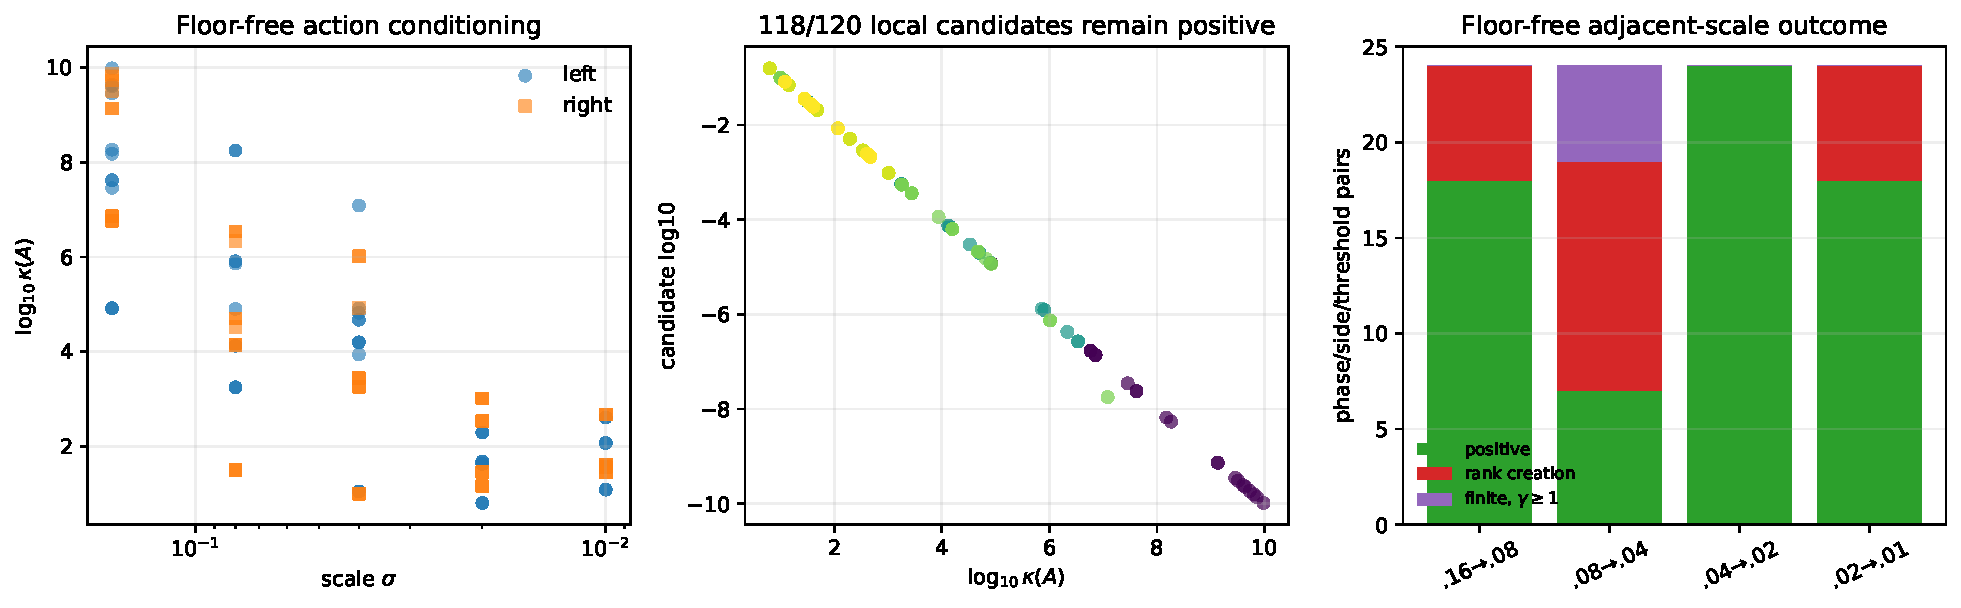
\includegraphics[width=\textwidth]{figures/floor_free_semidefinite_directional_audit.pdf}
\caption{Left: conditioning of all 120 floor-free actions.  Center: local
candidate size versus conditioning.  Right: the 96 adjacent-scale outcomes;
rank creation denotes an infinite exact-Gram tail factor.}
\label{fig:audit}
\end{figure}

\section{Results: local support survives, multiplicative chains do not}
All 120 recent actions have exact discrete rank four, and all 120 retain rank
four under the declared fp64 support radius.  The largest action condition
number is $10^{9.9844}$; the median logarithmic condition number is about
$3.25$.  These values explain why Gram eigenvalues seen in ordinary
precision can be much smaller---conditioning is squared by $A^*A$---but
they do not indicate actual loss of the fourth action direction.

The local Rayleigh calculation is also mostly stable under floor removal.
Exactly 118 of 120 states have $\gamma<1$ and therefore a positive
directional candidate.  Their candidate logarithms range from approximately
$-9.98$ to $-0.80$, with median about $-3.25$.  The two failures occur in
the left channel at $\sigma=0.08$, final phase, for thresholds $10^{-8}$
and $10^{-6}$; both have $\gamma\approx3.0719$.  Thus the five-scale data do
not support a claim that the local four-volume mechanism has disappeared.

The cross-scale conclusion is sharply different.  Of 96 adjacent pairs,
67 give a positive transferred lower bound.  Twenty-four have
$b_*=+\infty$ because the target tail has greater rank than the source tail.
Five additional pairs have finite $b_*$ but
$\sqrt{b_*}\gamma_{\rm source}\geq1$.  Every one of the 24 phase/side/
threshold chains contains at least one such blocked edge, so the complete
floor-free count is $0/24$, not the regularized $24/24$ reported in RH-125.

The obstruction is concentrated rather than random.  Six infinite factors
occur on the $0.16\to0.08$ edge, twelve on $0.08\to0.04$, and six on
$0.02\to0.01$.  The five finite superunit transfers all occur on
$0.08\to0.04$.  On the remaining $0.04\to0.02$ edge all 24 transfers are
positive.  This pattern is exactly what a changing finite-memory tail rank
should produce; it is not explained by loss of recent-action rank.

\section{Interpretation and revised route}
RH-130 changes the status of the directional route in two ways.  First, the
positive Gram floor in RH-121 was not needed to preserve recent-action rank
on the frozen data.  The four-dimensional local packet remains visible.
Second, the positive tail floor was mathematically consequential: it
converted forbidden rank-creating transitions into finite, sometimes
astronomical, multiplicative factors.  The maximum factor near
$10^{290}$ in RH-121 was therefore a warning sign, not merely an inconvenient
condition number.

The correct next recurrence is not
\[
 D_{n+1}\preceq b_nS_n^*D_nS_n
\]
but
\[
 D_{n+1}\preceq b_nS_n^*D_nS_n+F_n,
\]
where $F_n\succeq0$ covers tail directions born at the new scale.  After
normalization this is precisely the affine structure isolated in RH-123,
$\gamma_{n+1}^2\leq\rho_n\gamma_n^2+q_n$.  The immediate theoretical task
is therefore to characterize the minimal forcing on the support complement,
derive it from the memory recursion, and test whether $q_n$ is small enough
to coexist with eventual contraction.

This paper proves a finite-dimensional minimax theorem and a sharp
rank-creation obstruction, and it invalidates the interpretation of the
regularized five-scale chains as floor-stable evidence.  It does not prove
an all-level affine recurrence, a uniform bound on $\rho_n$ or $q_n$, a
positive normalized-base liminf, uniform Stage A, a Hilbert--Polya operator,
an identification of zeta zeros, or the Riemann Hypothesis.

\bibliographystyle{plainnat}
\bibliography{references}
\end{document}
